
\section{Interfaces}

\subsection{Mockup}

Figure 5.1 shows a mockup of the team analysis page that was created before starting developing. There is two main sections; Team statistics and key players

\begin{figure}[ht!]
\centering
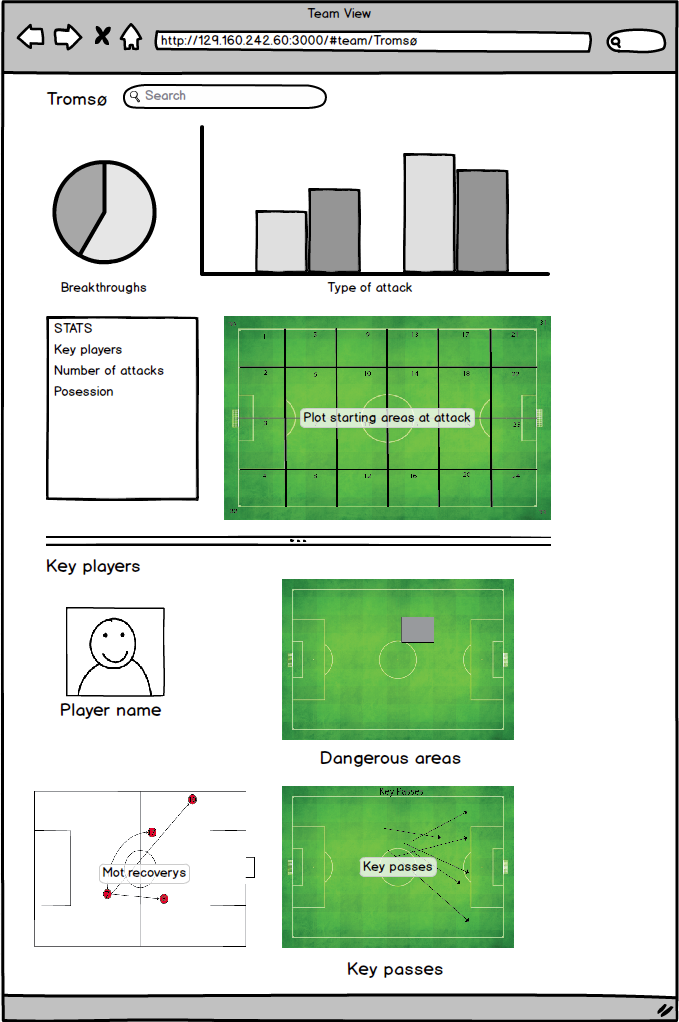
\includegraphics[width=150mm]{images/general/mockup.png}
\caption{All matches registrated in the database are listed on this page}
\label{overflow}
\end{figure}


\subsection{}

The first page you are prompted with is the listing of all matches registered in the database. A click on match gives you details about that match and prompts you a interface for capturing new attacks if requested. Every field has to be submitted with an correct input value.

\begin{figure}[ht!]
\centering
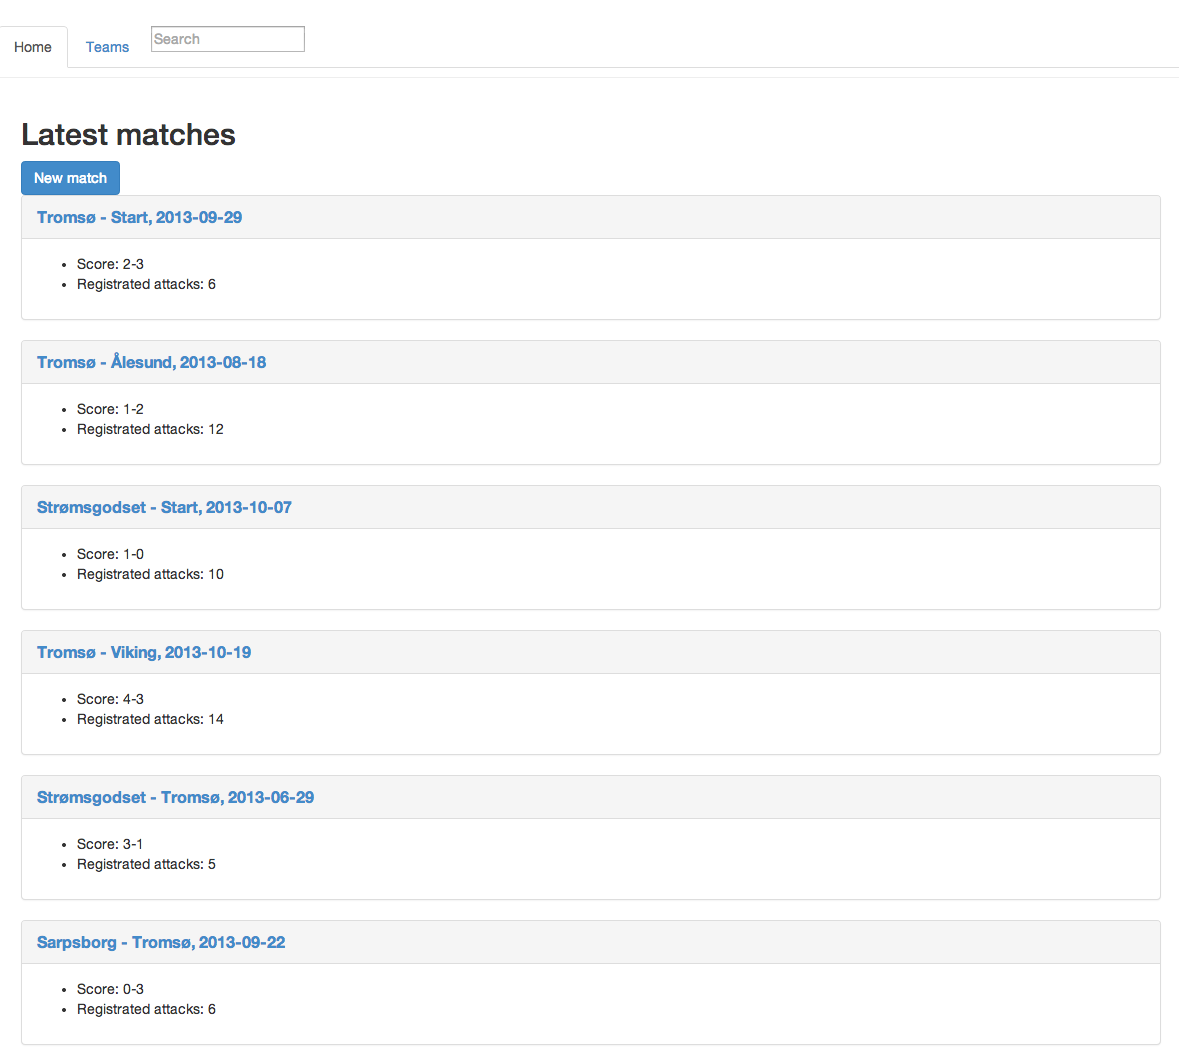
\includegraphics[width=100mm]{images/general/all_matches.png}
\caption{All matches registrated in the database are listed on this page}
\label{overflow}
\end{figure}


The whole web page follows a same theme throughout the pages. This theme is the standard theme in the CSS and JavaScript library Bootstrap (REF).  Bootstrap is also default responsive. This means the content on the site is automatically re-sized out from the size of your browser window.

You registrate a new attack by pressing the «New attack» button.  Here you fill in the result and date of the match.  When you submit the match you will be sent back to the home page. 

\begin{figure}[ht!]
\centering
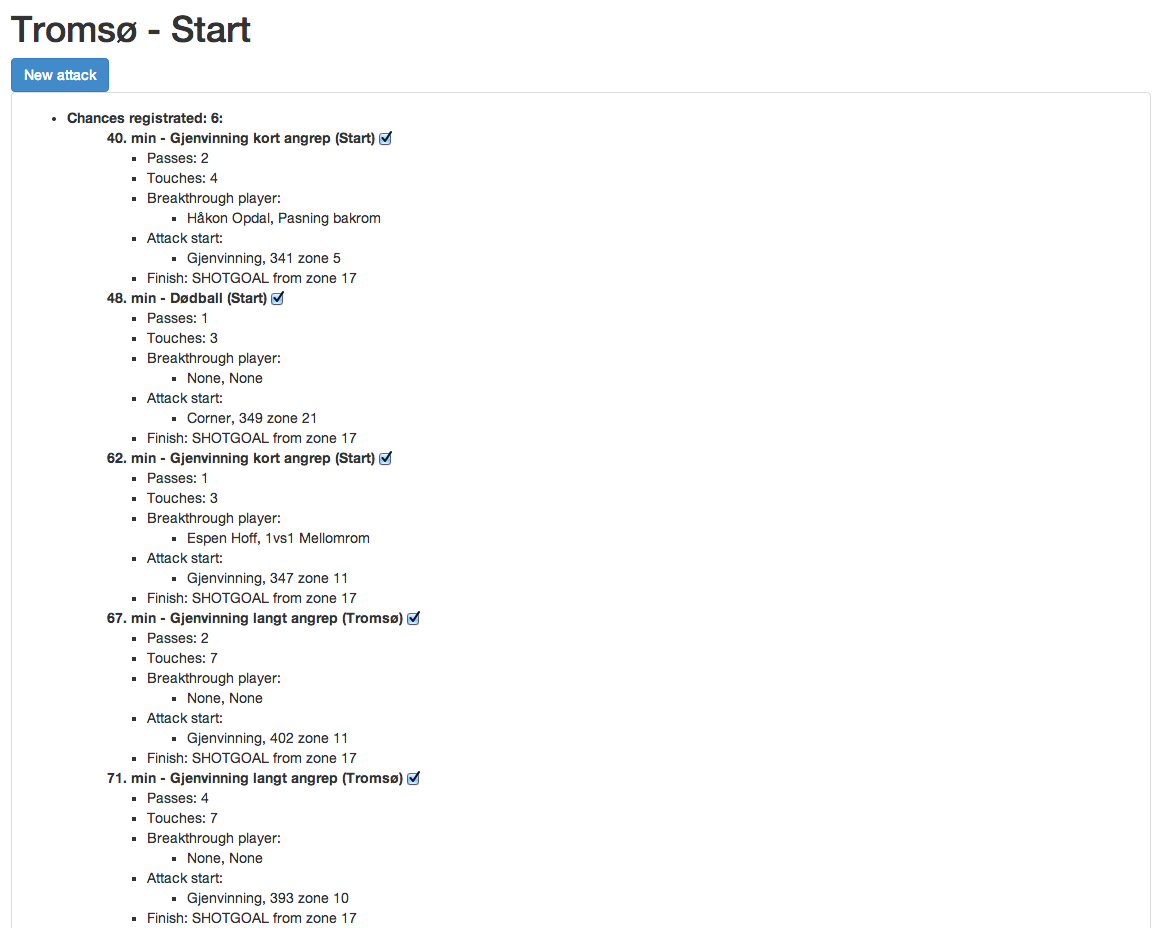
\includegraphics[width=80mm]{images/general/all_attacks.png}
\caption{Interface listing up all attacks for a match}
\label{overflow}
\end{figure}

Clicking on a match gives you overview of all attacks registrated for that particular game. This view is only meant for quality checking the data.
From the match you can registrate new attack attempts. This will prompt you with a fill in form for the attack. Attack start and attack end. Add the passes in the order they occur in the attack. 

\begin{figure}[ht!]
\centering
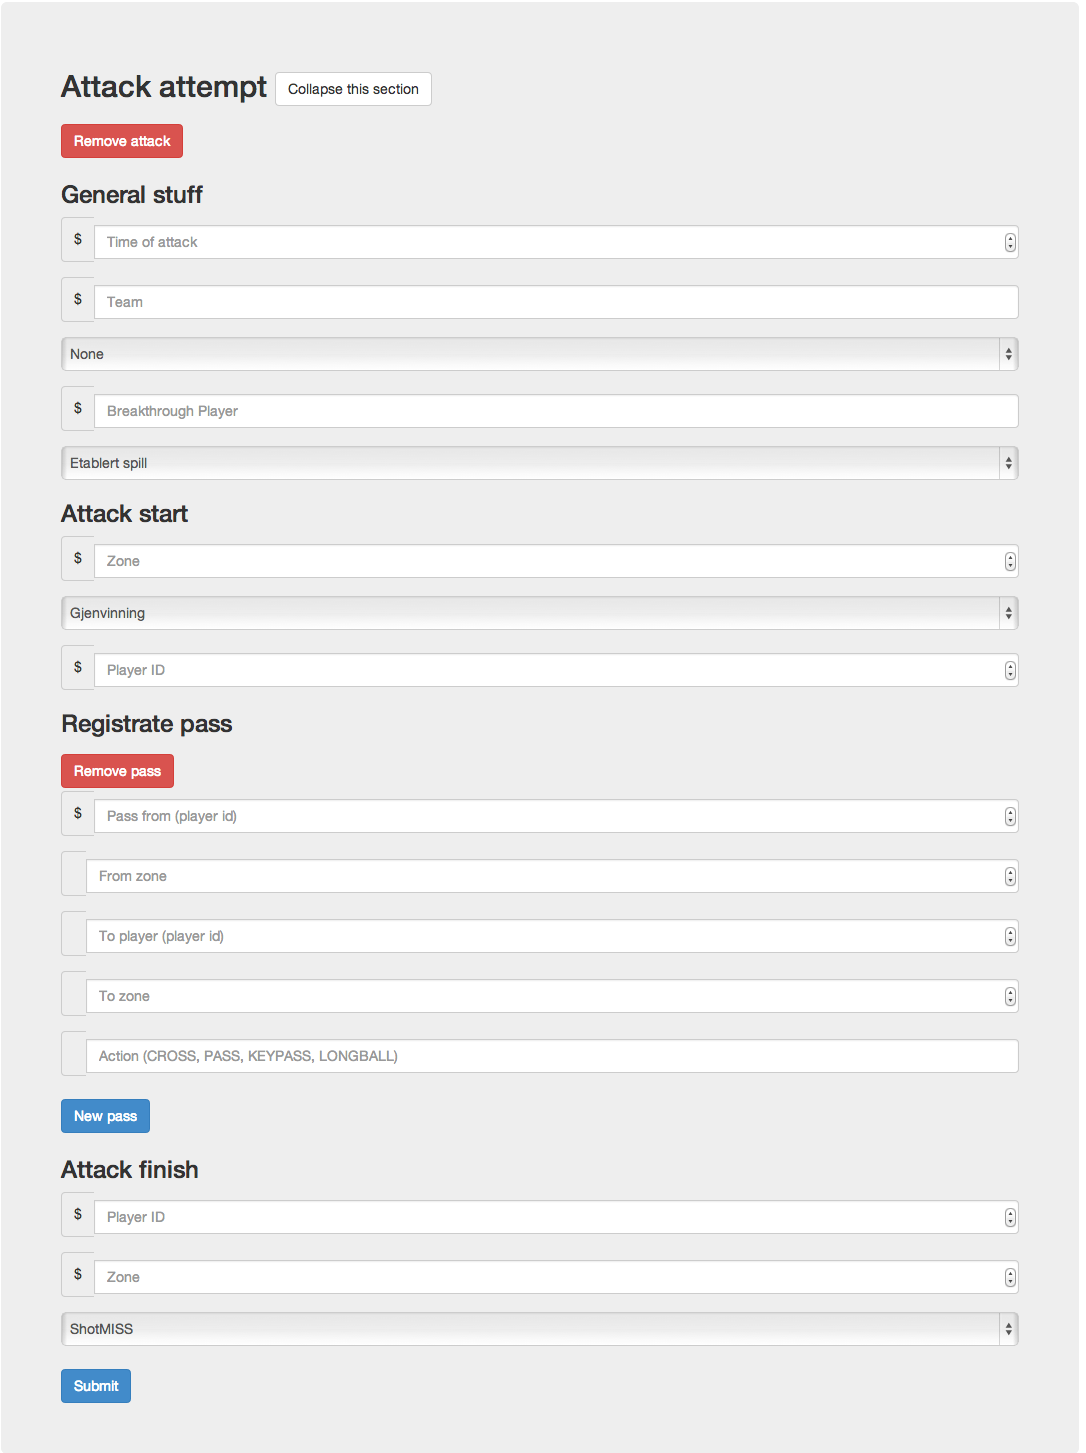
\includegraphics[width=80mm]{images/general/reg_attack.png}
\caption{Interface for registrating an attack}
\label{overflow}
\end{figure}

Then you have the team selection; a simple layout listing all the teams in the Norwegian premier league. From here you select the team you want to analyze.

\begin{figure}[ht!]
\centering
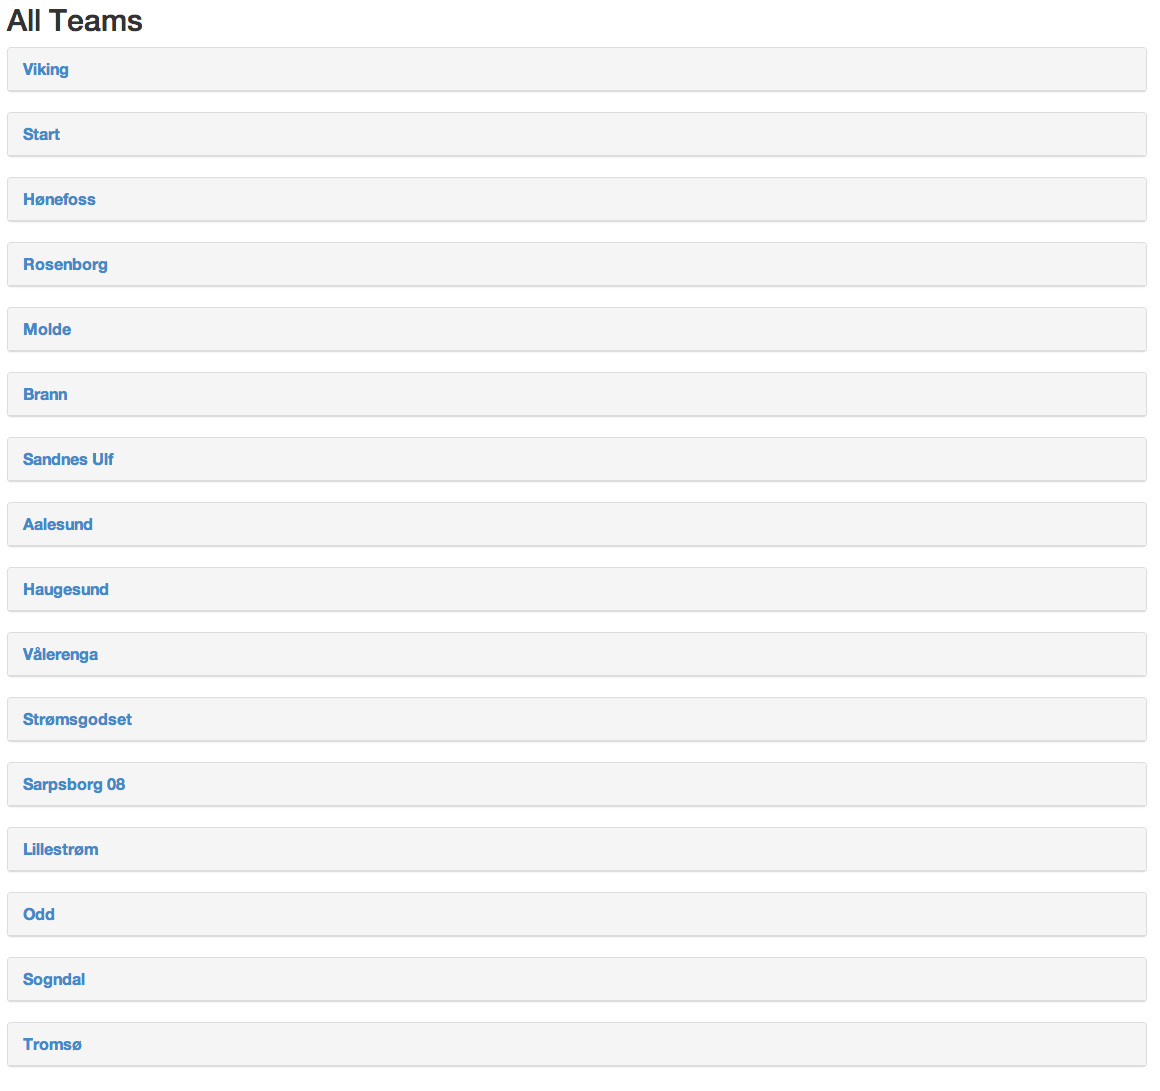
\includegraphics[width=80mm]{images/general/all_teams.png}
\caption{Interface listing all teams}
\label{overflow}
\end{figure}

Then there is the main view used for analyzing a team. The view is not the same as the mockup. This comes from a various things. A description of different breakthroughs has been added to enlighten users of the system. Users of the system may or may not have been in the process of capturing the data. In the mockup key players where highlighted. In the final view various statistics is presented to the user and he can then click on players he find interesting to know more about.  The whole page is divided into 3 sections; Key aspects, offensive play, defensive play.

\begin{figure}[ht!]
\centering
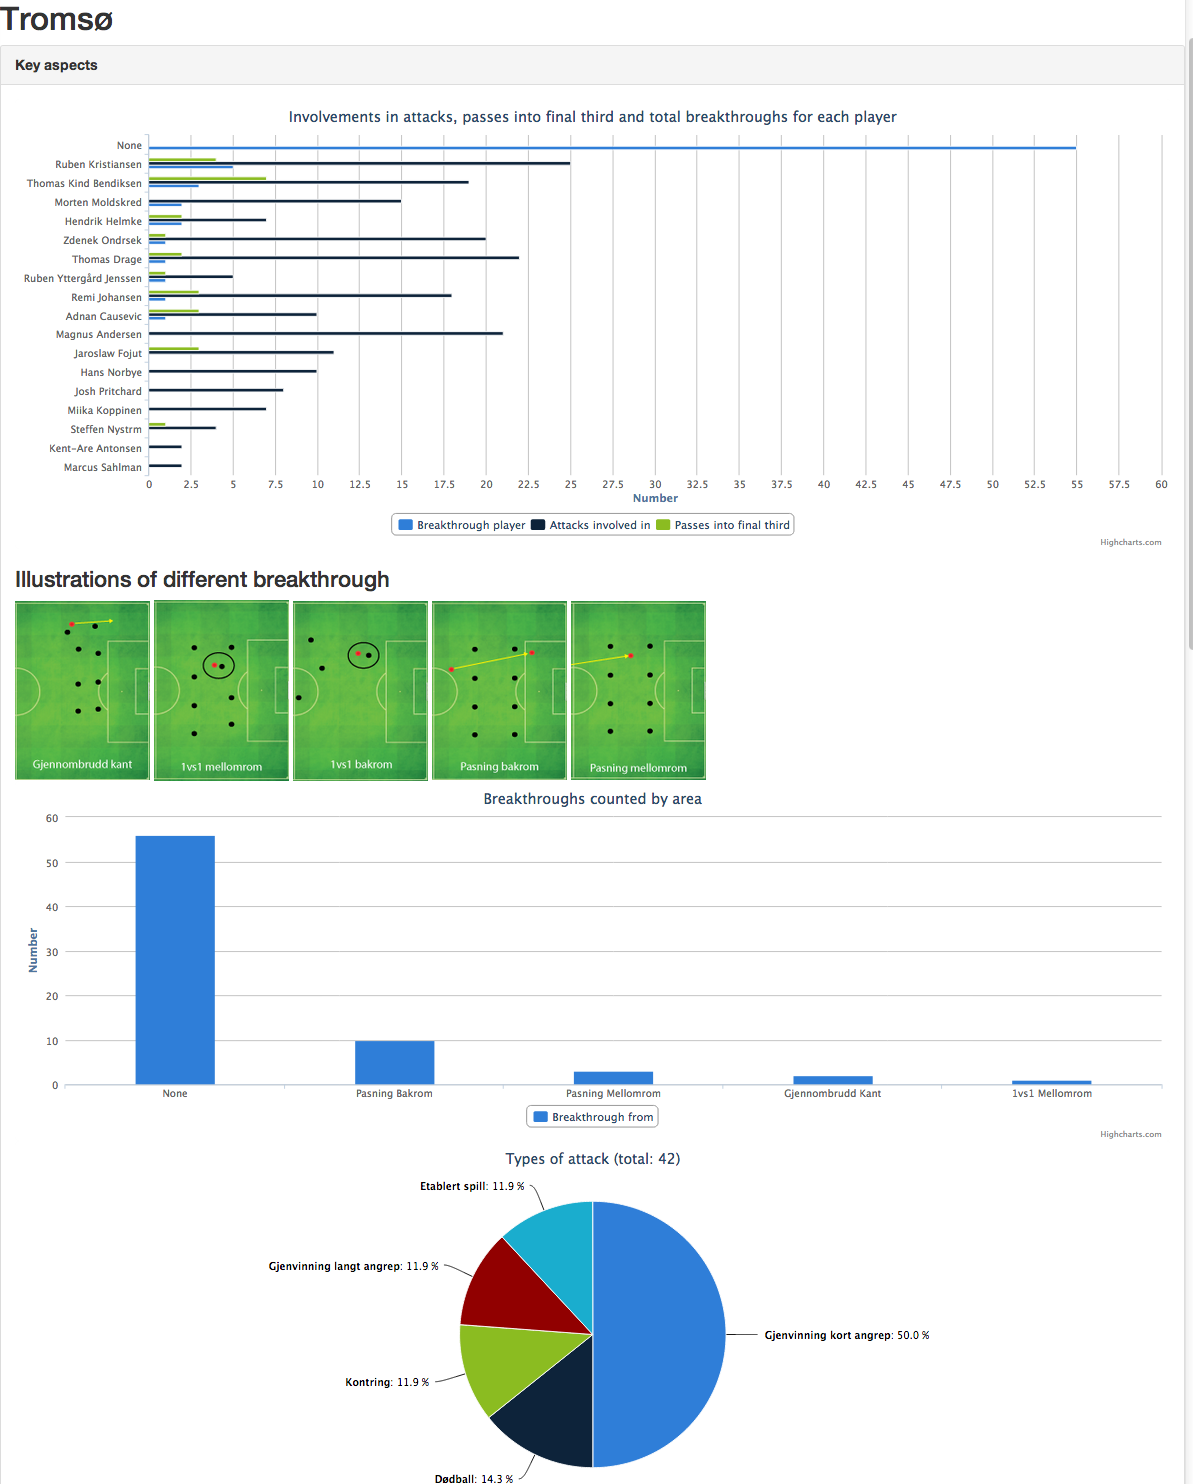
\includegraphics[width=80mm]{images/general/team_analysis1.png}
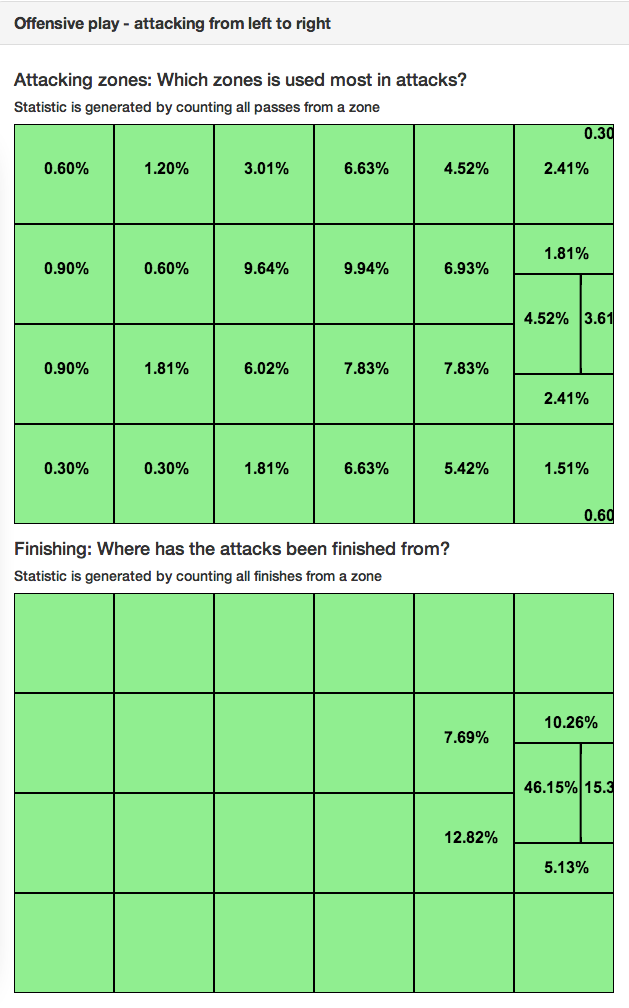
\includegraphics[width=80mm]{images/general/team_analysis2.png}
\caption{Main interface for information about opponents}
\label{overflow}
\end{figure}

Clicking on a player brings you to the player view. Here individual statistics is highlighted. 
